\chapter{Introduction}
\label{ch:intro}

\vspace{-2.5em}

\noindent In recent years, Multi-agent Reinforcement Learning (MARL) has experienced a significant surge in research activity, driven by the ongoing AI advancements and substantial funding dedicated to this field (\cite{gilbert2023reward}). The global market for MARL was valued at $2.8$ billion in 2022, with projections indicating a robust compound annual growth rate (CAGR) of $41.5\%$ from 2023 to 2032. By 2032, it is anticipated to soar to a remarkable $\$88.7$ billion (\cite{reinforcementLearningMarket2023}). Advancements in academic research indicate an upcoming trend where both implicit and explicit Reinforcement Learning (RL) systems will display heightened efficacy. These systems are poised to find more general applications in user-facing domains, delivering more significant impacts (\cite{kirk2023personalisation}).

\bigskip

\noindent A significant portion of contemporary research dedicates efforts to exploring emergent intelligence within cooperative environments, serving as a bridge between current research and the pursuit of Artificial General Intelligence (AGI) (\textcolor{deepblue}{\cite{lowe2020multiagent}; \cite{foerster2018learning}}). These studies center on environments that abstract real-world scenarios, characterized by interacting agents, diverse interests, varied goals, and the sharing of resources. Such environments inherently possess dynamism, displaying both evolving environmental conditions and fuzzy goal dynamics. Research has also demonstrated that competitive environments often foster heightened cooperation among agents (\textcolor{deepblue}{\cite{openai2019dota}; \cite{baker2020emergent}}). By utilizing multiple trajectories, the learning agent can gain experience from a wider array of interactions, with more players enhancing the diversity of trajectories encountered. In such settings, agent's objectives shift towards overcoming opposing teams, leading to continual refinement of policies until they surpass those of the opposing team. Competition inherently promotes dynamic interactions, devoid of a stable \textbdd{Nash equilibrium}, thereby promoting ongoing adaptation and the perpetual search to outwit the opposing team. Nash Equilibrium is a set of strategies, one for each player, such that no player has an incentive to deviate unilaterally from their strategy, given the strategies of the other players (\cite{doi:10.1073/pnas.36.1.48}; \cite{Nash1951}). In a zero-sum game, the gain of one participant is exactly offset by the losses of other participants, as the total amount of resources available is fixed. Therefore, any resource gained by one player directly results in a loss for another, defining the zero-sum nature of the environment. In such settings, a Nash equilibrium implies a situation where no player would benefit from changing their strategy. However, in reality, using this framework means that one player's gain is another's loss, reflecting the directly opposing payoffs. In 1928, John von Neumann proved the \textbdd{Minimax theorem}, which states that every finite, two-player, zero-sum game has an equilibrium that coincides with the Nash equilibrium (\textcolor{deepblue}{\cite{Neumann1928}; \cite{doi:10.1073/pnas.36.1.48}; \cite{Nash1951}; \cite{books/daglib/0023252}; \cite{SCHULMAN2019336}; \cite{LI202016932}}).

\bigskip

\noindent Current research efforts are further enhanced through crowd-funded or organization-sponsored MARL competitions, strategically designed to fulfill various objectives (\textcolor{deepblue}{\cite{suarez2019neural}; \cite{agapiou2023melting}}). Such collaboration yields advantageous outcomes: organizations streamline research and development expenditures, acquire access to esteemed RL specialists, and stimulate a creative momentum for participants, enabling ongoing learning and advancement within the field. 

\bigskip

\noindent Environments such as LuxAI (\textcolor{deepblue}{\cite{lux-ai-season-2}}), upon which our work is centered, introduce inherent dynamism stemming from the evolving population dynamics. This dynamism facilitates intricate social scenarios, necessitating a high degree of interdependence among collaborating agents. However, it also presents a challenge regarding the compatibility of standard reinforcement learning algorithms (\textcolor{deepblue}{\cite{wong2022deep}}), typically designed for single-agent or static environments. Furthermore, the calculation of rewards emerges as a critical research area, with prevailing solutions often adopting a global reward framework, sometimes called \textcolor{deepblue}{\texttt{perfectly-cooperative}} games (\textcolor{deepblue}{\cite{chen2023emergent}; \cite{agapiou2023melting}; \cite{ye2023global}; \cite{leroy2020qvmix}; \cite{suarez2019neural}}). This approach raises notable concerns, particularly in environments where actions that push the agents towards the predefined goal are infrequent. In such cases, the model risks reinforcing globally detrimental actions initiated by a single agent.

\bigskip

\noindent A MARL solution can be conceptualized along a spectrum of organizational paradigms (\textcolor{deepblue}{\cite{piccoli2023control}}). At one end of the spectrum, the single-brain approach centralizes decision-making, where a collective of agents is treated as a single entity. In this model, a global observation is used to generate a unified trajectory, and rewards are distributed based on collective outcomes, which can inadvertently reinforce negative behaviors. In contrast, a hybrid model utilizes local information from all agents to generate a single trajectory but incorporates a global reward system. 

\bigskip

\noindent Our research improves on this hybrid model by allocating rewards to individual agents or groups based on their specific contributions, thus creating a performance-based environment that operates at the individual or small group level. This approach involves dividing the environment's trajectories among agents or groups, allowing for the calculation of rewards, log probabilities, value estimates, advantages, and entropy for each unit or group. This method bootstraps the learning process by ensuring that rewards only reinforce positive behaviors early on. At the other end of the spectrum is the fully multi-agent approach, where each entity interacting with the environment is treated as an independent learning agent. This significantly complicates the learning process by creating trajectories of varied lengths, as entities may enter or exit the scene, or be destroyed. Consequently, gathering a consistent amount of experience for each entity becomes challenging, especially when some entities may only exist in the environment for a fraction of the time compared to others. This situation leads to computational inefficiencies and data sparsity. Our solution effectively addresses these challenges by offering a framework that mitigates the issues associated with both the single-brain and fully multi-agent approaches. Our research also focuses on evaluating these methodologies in dynamically changing environments and offers insights into addressing computational and emergent intelligence challenges without heavy reliance on domain-specific constraints or rigid rules.

\bigskip

\noindent Our \textbdd{key contributions} are the following:

\begin{itemize}[itemsep=1pt, parsep=0pt]

\item We conducted a novel \textbdd{benchmark study} comparing a broad array of contemporary reinforcement learning algorithms, including PPO, R-PPO, M-PPO, A2C, TRPO, DQN, QR-DQN, and ARS, to test their performance in a multi-agent environment. We evaluated the results and provided a general guideline on which algorithms to use in multi-agent systems.

\item We implemented a \textbdd{single-brain monolithic method as a baseline} for multi-agent reinforcement learning, employing widely used approaches from the literature such as global observations, global rewards, and a unified trajectory for all entities in the environment to assess their performance.

\item We expanded the approach into a \textbdd{hybrid model} by incorporating local observations and a distributed reward system, where entities in the environment received rewards commensurate with their individual or group performance. This modification demonstrated that a distributed reward system significantly enhances the learning process by preventing the reinforcement of negative behaviors early in training. Additionally, we improved on our methods by investigating potential improvements through various grouping methods, such as clustering, random grouping, and expedited training by retaining only the top $N$ performers in a set of trajectories, or opting for a random selection based on metrics such as rewards or advantage. We also showed results with reward assignments based on a combination of individual performance and contributions from a global pool, effectively integrating individual achievement with overall group success. 

\item In our work, we \textbdd{benchmarked our results against one of the baselines} from the Lux repository (\textcolor{deepblue}{\cite{luxai_s2-baseline-source}}) and demonstrated that our solution achieves convergence over 14 times faster, completing training in less than 20 minutes, compared to the original implementation which required two days on an A100, using up to 40GB of memory. In contrast, our approach was implemented on a single V100 and used significantly less memory.

\item As a result of our comprehensive exploration in the problem space, we also \textbdd{provide a general framework for developing a network architecture} tailored for multi-agent applications using one of the policy gradient methods, specifically PPO. We demonstrated that proper initialization and seeding are crucial for convergence, and the necessity of employing robust regularization techniques. Our findings also indicate a threshold in network depth beyond which further deepening does not yield performance improvements. Additionally, we outline effective strategies and best practices for implementing Multi-Agent PPO-based reinforcement learning.

\end{itemize}

\section{Outline}

\noindent Given the complexity involved in fully understanding the environment, problem space, advanced applications of reinforcement learning in multi-agent systems, and the development of a specialized neural network structure for this context, we aim to provide a concise overview. This will cover how we conceptualized the project, aspects that can be simplified or skipped, and how we have presented our results. The introduction section is structured as follows:

\begin{itemize}[itemsep=1pt, parsep=0pt]



\item \autoref{sec:background} introduces basic concepts of reinforcement learning elements, such as \textbdd{agent, policies, value functions, action-value functions, Bellman equations, states, rewards, discounted returns, episodes and optimality}. If the reader is familiar with these topics we recommend skipping to approximation methods (\autoref{sec:Policy-Gradient-Methods}).



\item \autoref{sec:Policy-Gradient-Methods} introduces concepts of \textbdd{policy gradient methods, actor-critic methods, value and policy approximator, value-based methods, value and policiy iterations, linear approximators, neural network approximators and evolutionary algorithms}. If the reader is familiar with these topics, we recommend skipping to to the description of the environment (\autoref{sec:environment}).



\item \autoref{sec:environment} introduces the rules of the \textbdd{Lux AI Competition}. If the reader comfortable with the environment, we recommend completely skipping the introductory section and going straight to the methods section (\autoref{ch:meth}).

\end{itemize}

\noindent The methods and results sections are closely integrated, with our findings presented in three distinct phases, as follows:

\begin{itemize}[itemsep=1pt, parsep=0pt]

\item \textbdd{Single Unit Testbench}: In the methods section, we introduce the novel reinforcement learning algorithms (\autoref{sec:trpo}) used for testing and provide an overview of the feature space, action space, and neural network architecture utilized in the benchmark (\autoref{sec:single-unit-testbench}). We also provide a detailed description of the training environment (\autoref{sec:single-unit-training}) and specific details regarding the evaluation processes (\autoref{sec:single-unit-eval}). The results section details the quantitative outcomes and conclusions drawn from these tests (\autoref{sec:single-unit-testbench-results}), helping us to select the most suitable algorithm for further studies in the subsequent sections.

\item \textbdd{Monolithic Approach}: We established a baseline using novel and contemporary research to create a simple, monolithic approach for our multi-agent reinforcement learning problem (\autoref{sec:monolithic-approach}). Utilizing the top-performing model from the single unit testbench, we expanded the scope to a multi-agent scenario (\autoref{sec:multi-agent-environment}) that includes multi-unit generation. This section proves particularly valuable as it serves as a benchmark; subsequent studies demonstrate significant enhancements over this single-brained method, highlighting the effectiveness of our research. We maintain consistent sections for training (\autoref{sec:monolithic-approach-training}), evaluation (\autoref{sec:monolithic-approach-eval}) and results (\autoref{sec:monolithic-approach-results}) within this monolithic approach.

\item \textbdd{Hybrid Approach}: This is the main novelty of our contribution which explores the expansion of the previously mentioned monolithic method towards a fully multi-agent approach. We incorporate features such as reward groupings, individual and group level trajectories, and calculations for rewards, values, and advantages (\autoref{sec:hybrid-approach}). The methods section in this phase also provides architectural recommendations and insights (\autoref{sec:hybrid-network-architecture}). The results are comprehensive (\autoref{sec:hybrid-approach-results}), including performance tests and ablation studies. For additional details on initialization techniques, seeding, and the limits of neural network architecture, we direct the reader to the discussion chapter, where we delve into less quantified findings from our research (\autoref{ch:disc-init-is-all-you-need}).

\end{itemize}

\section{Related Works}

\noindent In our review of related works, we'll explore solutions proposed during the competition to tackle multi-agent environments with dynamic entity numbers. We'll examine their unique features, discussing why certain approaches excel while others face challenges. This section will employ terminology specific to the Lux environment, which we'll introduce more briefly in \autoref{sec:environment}.

\noindent Numerous approaches to large multi-agent systems rely on logic systems characterized by extensive lines of code, meticulous fine-tuning to handle edge cases, and the accumulation of a comprehensive domain knowledge, upon which rule-based agents operate (\textcolor{deepblue}{\cite{du2024survey}; \cite{Aguayo_Canela_2021}}). Within the Lux Environment, several logic-based solutions have emerged, demonstrating notable success (\textcolor{deepblue}{\cite{ry_andy}; \cite{tigga}; \cite{kostuch}}). However, the primary drawback of these systems lies in their scalability, particularly in terms of code complexity and the interoperability of rules. Furthermore, the exponential growth in environment complexity significantly amplifies the number of edge cases that agents must account for. Reproducibility and comprehensibility of the code after inspection pose additional challenges due to the codebase often exhibiting a notoriously known anti-pattern called spaghetti code (\textcolor{deepblue}{\cite{Politowski_2020}}). These rule-based distributed agents were designed to prioritize efficient resource collection and allocation, employing alternating phases to effectively generate more resources than expended.

\bigskip

\noindent Data-driven methods like Imitation Learning have garnered attention in recent studies, thanks to the abundant hardware resources and investments (\textcolor{deepblue}{\cite{imit_learning}}). These techniques leverage learning from replay methods, allowing IL models to discern patterns from expert replays. These replays can originate from human-generated data or be acquired from larger models, resulting in more compact, distilled models. However, Imitation Learning demands substantial amounts of data and computational resources to operate efficiently (\textcolor{deepblue}{\cite{goecks2022combining}; \cite{garg2022iqlearn}}). Proposed methods within the Lux Environment have shown competitiveness but at significant costs, both in terms of training expenses and data acquisition (\textcolor{deepblue}{\cite{nagradov}}). Imitation Learning has also been used in neural network architecture search (\textcolor{deepblue}{\cite{ferdinand}}), resulting in three months of training and data collection time.

\bigskip

\noindent In the current landscape of deep learning and the large-scale era, deep reinforcement learning models of substantial size have set new benchmarks. For instance, models trained from scratch, such as AlphaGo Zero and GOAT, necessitate a considerable amount of computational power for training, with AlphaGo Zero requiring approximately 7.8e+13 GFLOPs (78 PetaFLOPs) and comprising over 46 million parameters, while GOAT has upwards of 35 million parameters (\textcolor{deepblue}{\autoref{fig:game-trends}}). Language models exemplify this trend even more starkly, with PalM2 possessing an unprecedented 340 billion trainable parameters (\textcolor{deepblue}{\cite{Sevilla_2022}}). 

\bigskip

\begin{figure}[htbp]
    \centering
    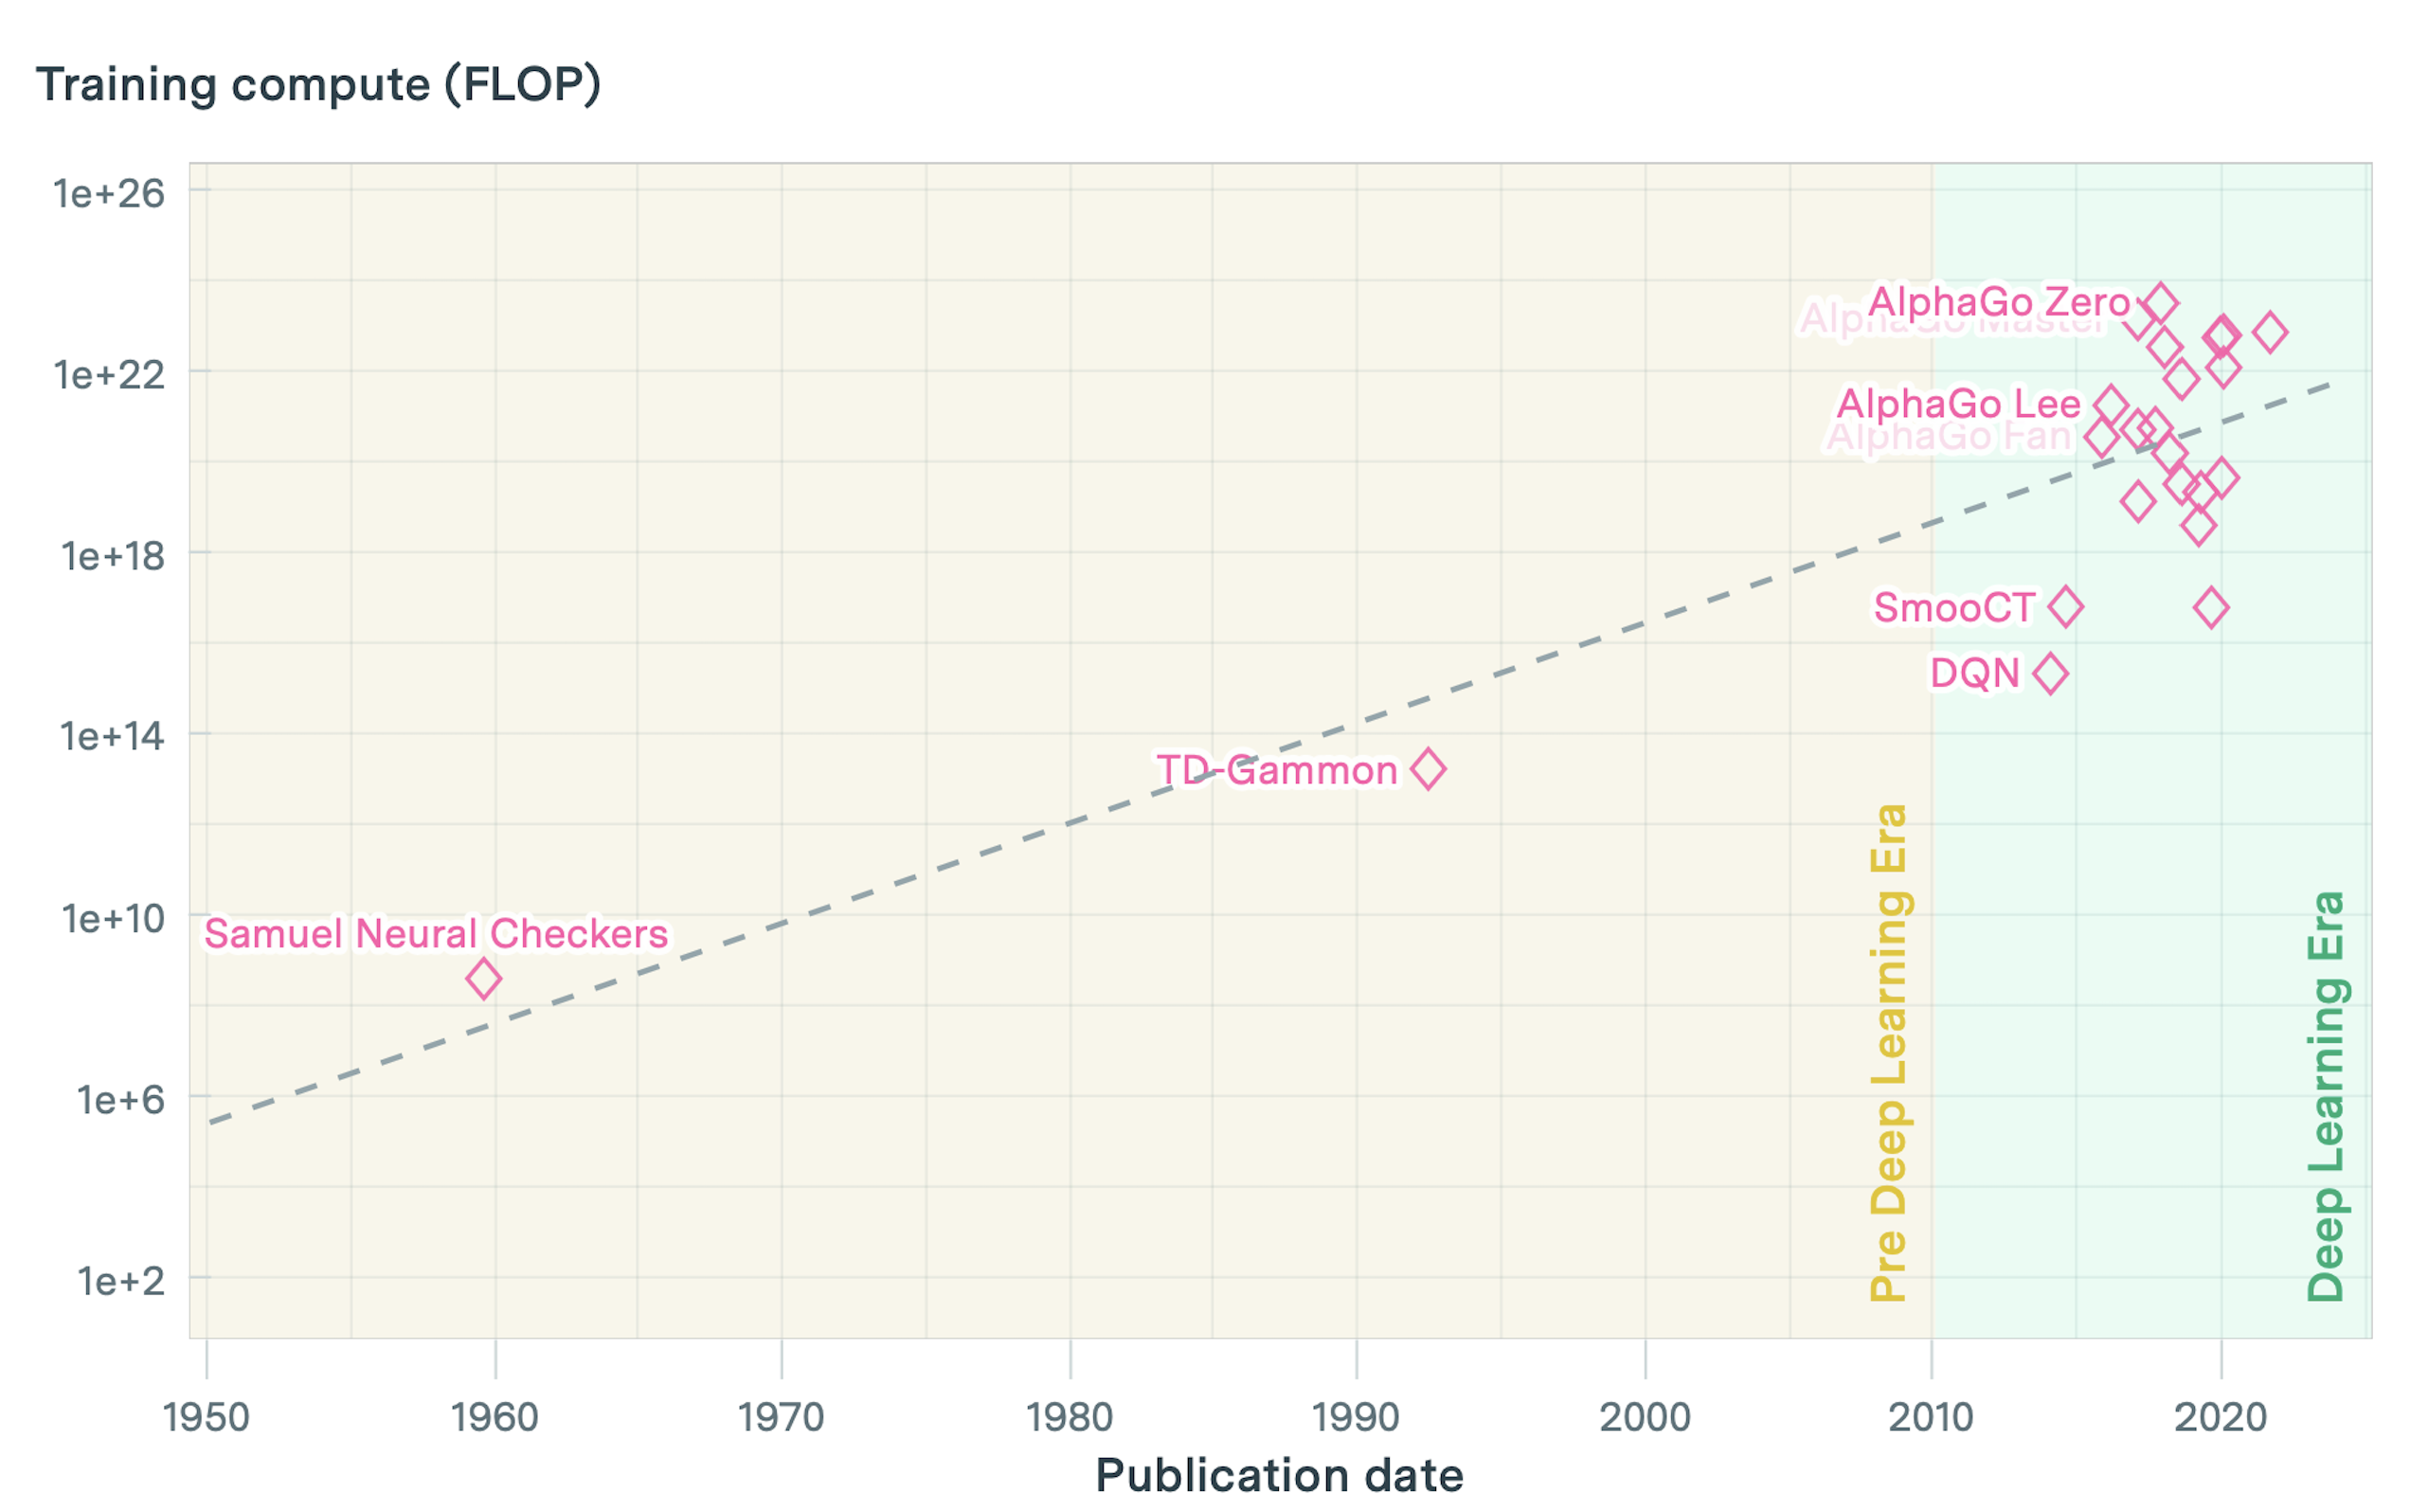
\includegraphics[width=1\linewidth]{images/intro/related_works/game-trends.png}
    \captionsetup{justification=justified, singlelinecheck=false, width=1\linewidth, labelfont=bf}     
    \caption{Exponential growth in training compute requirements for notable AI systems from the 1950s to the present, illustrating the transition from early machine learning to the current Large Scale Era (\textcolor{deepblue}{\cite{epoch2023pcdtrends}}).}
    \label{fig:game-trends}
\end{figure}

\noindent In the domain of complex, high-dimensional grid environments (\textcolor{deepblue}{\cite{eberhardinger2023learning}}), the deployment of deep neural networks is crucial for achieving effective generalization. This requirement is particularly pronounced in the context of the Lux environment, where map heterogeneity is guaranteed by design, where the generation of different environments is seed-dependent. To tackle these issues, (\textcolor{deepblue}{\cite{chen2023emergent}}) proposed a large-scale deep learning solution designed to analyze a wide-ranging, high-dimensional feature space, incorporating diverse environmental attributes like ore maps, ice maps, and distances. They introduced a comprehensive global reward system aimed at recognizing and rewarding any positive developments of an agent, thereby achieving a highly generalized model capable of adapting across various scenarios. This approach necessitated substantial computational resources, specifically requiring an V100 GPU and an additional 600 CPU cores, with the training process extending over multiple phases spanning several days.

\bigskip

\noindent Recent advancements include a deep reinforcement learning algorithm specifically engineered for the complexity of industrial multi-agent systems. Addressing a gap in the research, their approach, the K-nearest multi-agent deep RL (\textcolor{deepblue}{\cite{khorasgani2022knearest}}), is designed to handle scenarios with a fluctuating number of agents and action dependencies among them. Demonstrated through a fleet management simulation by Hitachi, their algorithm showed potential for significant improvements in productivity by optimizing collaborative tasks, such as traffic management, highlighting its applicability in dynamic industrial environments. The paper by (\textcolor{deepblue}{\cite{min2024dynamic}}) presents a novel approach in multi-reward reinforcement learning focused on generating counselor reflections. They introduce two innovative bandit methods, DynaOpt and C-DynaOpt (\textcolor{deepblue}{\cite{min2024dynamic}}), for dynamically adjusting reward weights during training, aiming to optimize text qualities. Their methods outperform existing models, demonstrating significant potential for multi-objective problem decomposition and dynamic rewarding systems. (\textcolor{deepblue}{\cite{Tan_2024}}) propose an adaptive distributed reinforcement learning method for multi-objective optimization in dynamic, distributed Intelligent Transportation Systems. Their approach addresses the challenge of optimizing multiple, potentially conflicting objectives in a changing environment by integrating multi-agent reinforcement learning with adaptive few-shot learning. Tested in an ITS scenario, their algorithm demonstrates superior adaptation and performance across individual and system metrics. (\textcolor{deepblue}{\cite{zheng2024multiagent}}) introduce a novel approach in Multi-Agent Reinforcement Learning (MARL) employing a hierarchy of Reward Machines (RMs) to enhance learning efficiency in cooperative tasks. Their method, MAHRM, adeptly manages complex scenarios with concurrent events and interdependent agents by breaking down tasks into simpler sub-tasks. 


\section{Background}
\label{sec:background}

\noindent Reinforcement Learning (RL) encapsulates all the processes through which agents learn optimal behaviors through exploration and the evaluation of actions based on rewards and penalties. This framework excels in single-agent, single-objective optimization scenarios because it directly aligns an agent's learning process with the maximization (or minimization) of a specific goal, enabling the agent to iteratively refine its strategy towards achieving optimal performance in well-defined environments (\textcolor{deepblue}{\cite{Lee_2020}}). Exploring advanced Reinforcement Learning topics necessitates a solid grasp of the fundamental RL concepts due to the technical complexity of the field. Specifically, Policy Optimization algorithms, which extend basic RL principles, are detailed and form the basis for further discussion. This discourse selectively highlights relevant concepts, omitting details beyond the scope of our research. For a thorough foundational understanding, the seminal work "Reinforcement Learning: An Introduction" by Sutton and Barto (\textcolor{deepblue}{\cite{Sutton1998}}) is an essential reference.

\bigskip

\begin{figure}[htbp]
    \centering
    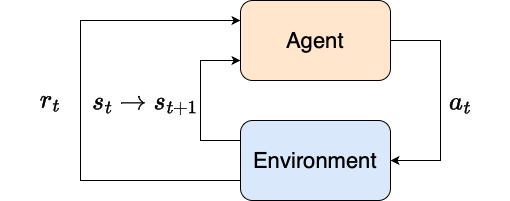
\includegraphics[width=0.6\linewidth]{images/intro/background/rl_simple.png}
    \captionsetup{justification=justified, singlelinecheck=false, width=1\linewidth, labelfont=bf}  
    \caption{The standard representation of the agent-environment control loop depicts the agent as the actuator and the environment as a sensor, sending signals to this actuator. These signals typically consist of reward signals, reflecting the efficacy of the agent's last action $a_t$, and a new environment signal $s_{t+1}$, updated based on the agent's actuator action $a_t$.}
    \label{fig:rl_simple}
\end{figure}

\noindent In reinforcement learning, the foundational components are the \textbdd{environment} and the \textbdd{agents} operating within it. Agents interact with the environment by executing actions informed by \textbdd{observations}, which may vary in terms of their completeness and detail. Based on these observations, the agent decides on \textbdd{actions}, influencing the environment, which can also change independently. The agent aims to maximize its \textbdd{total rewards} over time, known as the return, by learning optimal actions through its interactions. Reinforcement learning techniques enable this learning process by guiding the agent to achieve its goal of reward maximization.

\bigskip

\noindent In deep reinforcement learning, a state $s$ is a detailed representation of the environment, containing all pertinent information, while an observation $o$ provides a subset of this information, possibly omitting crucial details. Deep RL frameworks typically use vectors, matrices, or tensors to model these states and observations. For example, an image might be represented by its RGB values, and a robot's status by vectors of its joint angles and velocities. The environment's \textbdd{observability} is classified based on the agent's access to information: it is fully observed if the agent perceives the entire state, and partially observed if the agent only gets incomplete observations. We will not consider partial observability, since our work focuses only on a fully observed environment (\autoref{sec:environment}).

\bigskip

\noindent The \textbdd{action space} of an environment defines all possible actions an agent can execute. Environments may feature \textbdd{discrete} action spaces, where the choices are finite and distinct (\textcolor{deepblue}{\cite{mnih2013playing}; \cite{SilverHuangEtAl16nature}}), or \textbdd{continuous} action spaces, characterized by actions as real-valued vectors that offer a spectrum of possibilities. This research explores an environment that integrates both discrete and bounded continuous actions (\autoref{sec:environment}; \autoref{fig:lux-actions_ex}).

\bigskip

\noindent Regarding the actions available to the agent, we define the concept known as a \textbdd{policy}. Policies may be \textbdd{deterministic}, implying that, for a given state, the action selected is consistent and not derived from a probability distribution of actions (\textcolor{deepblue}{\cite{Sutton1998}; \autoref{eq:deterministic-policy}}) .

\begin{equation}
    a_t = \mu(s_t)
    \label{eq:deterministic-policy}
\end{equation}

\noindent The chosen action can be \textbdd{stochastic}, derived by sampling from a probability distribution over possible actions (\textcolor{deepblue}{\cite{Sutton1998}; \autoref{eq:stochastic-policy}}).

\begin{equation}
    a_t \sim \pi_{\theta}(\cdot | s_t).
    \label{eq:stochastic-policy}
\end{equation}

\noindent In deep reinforcement learning we are dealing with prameterized policies, which are characterized by their outputs being computable functions reliant on a distinct parameter set, such as the weights inside an \textbdd{artificial neural network} (ANN), that we can adjust dynamically to the modify the actions of the agent via optimization methods. These weights are usually denoted by $\theta$ (\textcolor{deepblue}{\autoref{eq:stochastic-policy}}). In our research, we exclusively focus on stochastic policies to facilitate exploration; hence, discussions on deterministic policies are beyond the scope of this research.

\bigskip

\noindent The two primary stochastic policies implemented in current deep reinforcement learning frameworks are \textbdd{categorical} and \textbdd{diagonal Gaussian policies} (\textcolor{deepblue}{\cite{SpinningUp2018}}). Categorical policies are designed for discrete action spaces. Diagonal Gaussian policies, on the other hand, are appropriate for continuous action spaces. The Lux Environment utilizes discrete and bounded continuous action values within its action space (\autoref{sec:environment}; \autoref{fig:lux-actions_ex}), but for the purposes of simplification, we used a discretization technique known as \textbdd{binning}. This approach significantly improves performance in on-policy optimization (\textcolor{deepblue}{\cite{tang2020discretizing}}), allowing action prediction in continuous domains using categorical policies. These policies serve as classifiers within the action selection mechanisms, utilizing a neural network to process inputs and ending with a linear layer that generates \textbdd{logits} for each possible action. Logits represent the unnormalized scores output by the linear layer, which are then converted into a probabilistic distribution of actions through the softmax function.

\bigskip

\noindent A \textbdd{trajectory} (\textcolor{deepblue}{\cite{Sutton1998}; \autoref{eq:trajectory}}) represents a sequence composed of state-action pairs as experienced within the environment.

\begin{equation}
    \tau = (s_0, a_0, s_1, a_1, \hdots).
    \label{eq:trajectory}
\end{equation}

\noindent Typically, the initial state of the environment is drawn from a \textbdd{starting state distribution} (\textcolor{deepblue}{\cite{Sutton1998}; \autoref{eq:start-state-distrib}}).

\begin{equation}
    s_0 \sim \rho_0(\cdot).
    \label{eq:start-state-distrib}
\end{equation}

\noindent State transitions within an environment are dictated by the environment's inherent dynamics and depend on the previous action executed, represented by $a_t$. These transitions may follow a deterministic or stochastic pattern, as highlighted in (\textcolor{deepblue}{\cite{Sutton1998}; \autoref{eq:transition}}). 

\begin{equation}
    s_{t+1} \sim P(\cdot | s_t, a_t).
    \label{eq:transition}
\end{equation}

\noindent Specifically, the Lux Environment runs under deterministic rules, as detailed in \autoref{sec:environment}, ensuring that each action directly results in a predictable environmental update. Moving forward, we will term trajectories as \textbdd{rollouts}, adopting a standard nomenclature used in RL.

\bigskip

\noindent The reward function, represented by $R$ has diverse notational variations, with a common formulation involving the agent's current state, the action executed in that state, and the subsequent state resulting from the action (\textcolor{deepblue}{\cite{Sutton1998}; \autoref{eq:reward}}).

\begin{equation}
    r_t = R(s_t, a_t, s_{t+1})
    \label{eq:reward}
\end{equation}

\noindent The notation for reward is often simplified to depend solely on the state at timestep $t$, $R(s_t)$, or on both the current state and the recently executed action at timestep $t$, $R(s_t, a_t)$. The objective of the agent is to maximize the total accumulated reward throughout a rollout, denoted as $R(\tau)$ (\textcolor{deepblue}{\cite{Sutton1998}}). However, given the variety of possible returns, this notation can be ambiguous. The first concept of return encountered in the literature is termed the \textbdd{finite-horizon undiscounted return}, which aggregates the rewards collected within a predetermined rollout window (\textcolor{deepblue}{\cite{Sutton1998}; \autoref{eq:reward-undiscounted}}).

\begin{equation}
    R(\tau) = \sum_{t=0}^{T} r_t.
    \label{eq:reward-undiscounted}
\end{equation}

\noindent  Mathematically, the reward may not always converge to a finite value. To address this, the concept of \textbdd{infinite-horizon discounted return} is introduced, which applies a discount factor, $\gamma$ to future rewards. This discounting ensures convergence under suitable conditions. When $\gamma$ is set to 1, it results in the equivalent of an undiscounted return (\textcolor{deepblue}{\cite{Sutton1998}; \autoref{eq:reward-discounted}}).

\begin{equation}
    R(\tau) = \sum_{t=0}^{\infty} \gamma^{t}r_t.
    \label{eq:reward-discounted}
\end{equation}

\noindent The core goal of the agent is to adopt a policy that ensures the maximization of its expected return, regardless of the specific return metric or policy model used. In a deterministic environment, such as the one addressed in our research, the probability function $P(s_{t+1} | s_t, a_t)$ transforms into a deterministic relation $s_{t+1} = f(s_t, a_t)$. This modification indicates that state transitions are directly determined by the current state and action, simplifying the calculation of trajectory probabilities under a given policy $\pi$ (\textcolor{deepblue}{\cite{Sutton1998}; \autoref{eq:prob-func}}).

\begin{equation}
    P(\tau | \pi) = \rho_0(s_0)\prod_{t=0}^{T-1} \pi(a_t|s_t).
    \label{eq:prob-func}
\end{equation}

\noindent Given that the transitions are deterministic, the expectation of the return, $J(\pi)$, remains (\textcolor{deepblue}{\cite{Sutton1998}; \autoref{eq:expected-return}}):

\begin{equation}
    J(\pi) = \int_{\tau} P(\tau | \pi) R(\tau) = \mathbb{E}_{\tau \sim \pi} \text{ }[R(\tau)]
    \label{eq:expected-return}
\end{equation}

\noindent The optimization challenge in reinforcement learning involves identifying the \textbdd{optimal policy} by selecting the argument $\pi$ that maximizes the expected return (\textcolor{deepblue}{\cite{Sutton1998}; \autoref{eq:optimal-policy}}).

\begin{equation}
    \pi^* = \arg \max_{\pi} J(\pi),
    \label{eq:optimal-policy}
\end{equation}

\noindent with $\pi^*$ being the optimal policy.

\bigskip

\noindent \textbdd{Value functions} quantify expected rewards from given states or state-action pairs under defined policies. Value functions estimate the benefit of an agent being in a specific state and play a role, in some form, across nearly all reinforcement learning algorithms (\textcolor{deepblue}{\cite{SpinningUp2018}; \cite{AlMahamid_2021}}). The \textbdd{On-Policy Value Function} calculates the expected reward for being in state $s$ while following a specific policy $\pi$, essentially computing the expected reward across a trajectory $\tau$ (\textcolor{deepblue}{\cite{Sutton1998}; \autoref{eq:value}}).

\begin{equation}
    V^{\pi}(s) = \mathbb{E}_{\tau \sim \pi} \text{ }[R(\tau) | s_0 = s]
    \label{eq:value}
\end{equation}

\noindent The \textbdd{On-Policy Action-Value Function} estimates the value of starting in state $s$, taking an initial arbitrary action $a$, and thereafter adhering to policy $\pi$, providing a measure that parallels the On-Policy Value Function but starts with a specific action $a$ (\textcolor{deepblue}{\cite{Sutton1998}; \autoref{eq:action-value}}).

\begin{equation}
    Q^{\pi}(s, a) = \mathbb{E}_{\tau \sim \pi} \text{ }[R(\tau) | s_0 = s, a_0 = a]
    \label{eq:action-value}
\end{equation}

\noindent \textbdd{Optimal value functions} signify the maximum expected return obtainable from a state $s$ when following the optimal policy within an environment. Conversely, optimal action-value functions indicate the highest expected return achievable by executing an action $a$ in state $s$ and adhering to the optimal policy for all subsequent decisions. The optimal value function is defined as (\textcolor{deepblue}{\cite{Sutton1998}; \autoref{eq:optimal-value}}):

\begin{equation}
    V^{*}(s) = \underset{\pi}{\text{max }} \mathbb{E}_{\tau \sim \pi} \text{ }[R(\tau) | s_0 = s],
    \label{eq:optimal-value}
\end{equation}

\noindent while the optimal action-value function has the following form (\textcolor{deepblue}{\cite{Sutton1998}; \autoref{eq:optimal-action-value}}):

\begin{equation}
    Q^{*}(s, a) = \underset{\pi}{\text{max }} \mathbb{E}_{\tau \sim \pi} \text{ }[R(\tau) | s_0 = s, a_0 = a].
    \label{eq:optimal-action-value}
\end{equation}

\noindent In value and action-value functions, we assume an \textbdd{infinite-horizon discounted return} to ensure convergence. Without discounting, a finite horizon is required to avoid infinite returns, making the concept of expected return meaningless and impractical for RL tasks. In the undiscounted case, incorporating time as an argument is necessary to account for time-dependence. An equally important connection in literature is to define the value function in terms of the action-value function (\textcolor{deepblue}{\cite{Sutton1998}; \autoref{eq:act-val-1}; \autoref{eq:act-val-2}}), highlighting their integral relationship. The value function using the action-value function is defined as:

\begin{equation}
    V^{\pi}(s) = \mathbb{E}_{a \sim \pi} \text{ }[Q^{\pi}(s, a)]
    \label{eq:act-val-1}
\end{equation}

\noindent while the optimal value function using the optimal action-value function has the following form:

\begin{equation}
    V^{*}(s) = \underset{\text{a}}{\text{max }} [Q^{*}(s, a)]
    \label{eq:act-val-2}
\end{equation}

\noindent \textbdd{The Bellman Equations}, crucial to reinforcement learning, establish a recursive linkage between the value of a specific state and the values of its ensuing states. They assert that the optimal policy at any stage matches the optimal policy at all future stages, effectively stating that the value of a state equals the immediate reward plus the expected value of next states under the optimal policy. This principle ensures the consistency and optimality of decision-making across time. Bellman equations use \textbdd{on-policy} notation (\textcolor{deepblue}{\cite{Sutton1998}; \autoref{eq:bellman-value}; \autoref{eq:bellman-action-value}}), calculating state values or action-values based on a specified policy $\pi$ \protect \footnotemark. 

\footnotetext{This notation sometimes leads to confusion with the concepts of on-policy and off-policy learning. In off-policy scenarios, though the equations appear similar, the policy $\pi$ refers to the target policy, whereas data collection follows a different behavior policy $\mu$.}

\begin{equation}
    V^{\pi}(s) = \mathbb{E}_{\underset{s' \sim P(\cdot | s, a)}{a \sim \pi(\cdot | s)}} \text{ } [r(s,a) + \gamma V^{\pi}(s')]
    \label{eq:bellman-value}
\end{equation}

\begin{equation}
    Q^{\pi}(s, a) = \mathbb{E}_{s' \sim P(\cdot | s, a)} [r(s,a) + \gamma \text{ } \mathbb{E}_{a' \sim \pi(\cdot | s')} \text{ } Q^{\pi}(s', a')]
    \label{eq:bellman-action-value}
\end{equation}

\noindent For both value iteration and policy iteration algorithms, the Bellman equations ensure convergence to the optimal policy (\textcolor{deepblue}{\cite{Sutton1998}}), given enough iterations and under certain conditions, such as a finite state space or the presence of a discount factor in infinite horizons. The Bellman equations for optimal value and action-value functions resemble the on-policy framework, yet differ in action selection. Instead of sampling actions a from a state-dependent probability distribution, the optimal framework selects the action that maximizes the future value (\textcolor{deepblue}{\cite{Sutton1998}; \autoref{eq:bellman-optimal-value}; \autoref{eq:bellman-optimal-action-value}}).

\begin{equation}
    V^{*}(s) = \underset{\text{a}}{\text{max }} \mathbb{E}_{s' \sim P(\cdot | s, a} \text{ } [r(s,a) + \gamma \text{ }V^{*}(s')]
    \label{eq:bellman-optimal-value}
\end{equation}

\begin{equation}
    Q^{*}(s, a) = \mathbb{E}_{s' \sim P(\cdot | s, a)} [r(s,a) + \gamma \underset{\text{a'}}{\text{ max }} \mathbb{E}_{a' \sim \pi(\cdot | s')} \text{ } Q^{*}(s', a')]
    \label{eq:bellman-optimal-action-value}
\end{equation}

\noindent In modern RL algorithms, the calculation of a so-called \textbdd{advantage function} plays a crucial role in optimal decision making. The advantage function quantifies the benefit of selecting a particular action $a$ in state $s$ compared to the average result of pursuing other available actions in the same state, given adherence to policy $\pi$ subsequently. The on-policy advantage function, $A^{\pi}(s, a)$, measures the expected benefit of choosing action $a$ compared to following the policy's action distribution in state $s$. This calculation involves subtracting the value function, representing the average benefit of being in state $s$, from the action-value function for a specific action $a$, thus determining a relative improvement over other actions (\textcolor{deepblue}{\cite{Sutton1998}; \autoref{eq:advantage}}). 

\begin{equation}
    A^{\pi}(s, a) = Q^{\pi}(s, a) - V^{\pi}(s)
    \label{eq:advantage}
\end{equation}

\noindent Our research environment (\autoref{sec:environment}) can be formulated as a fully-observable \textbdd{Markov Decision Process}, which is a formal notation frame work for an agent's environment. It is mathematically represented to indicate adherence to the Markov property, meaning that state transitionts do not rely on past history. At any given timestep $t$, the next state $s_{t+1}$ is influenced by the current state $s_t$ and the action $a_t$ taken at that state. In our study, we model our environment as an MDP (\textcolor{deepblue}{\cite{SpinningUp2018}}), represented by the tuple $\langle S, A, R, P, \rho_0 \rangle$, where:

\vspace{-5pt}

\begin{itemize}[itemsep=1pt, parsep=0pt]
    \item $S$ is the set of all possible states, including map features, units, and resources.
    \item $A$ encompasses the entire set of allowable actions, such as digging and moving.
    \item $R : S \times A \times S \rightarrow \mathbb{R}$ is the reward function, devised based on a specific reward scheme.
    \item $P : S \times A \times A_{adv} \rightarrow P(S)$ denotes the state transition probability function. This function is characterized as stochastic in adversarial environments. Transforming the setting to a cooperative scenario, or making the adversary passive, results in a deterministic transition probability of 1.
    \item $\rho_0$ represents the starting state distribution, determined by a controlled seeding method.
\end{itemize}

\noindent Modern RL algorithms fit into a diverse range of domains and applications. Our research focuses on \textbdd{model-free methods}, which operate without an explicit environmental model, restricting the ability to predict state transitions and rewards. This absence prevents the utilization of lookahead or planning techniques to enhance policy learning through forward simulation. Consequently, model-free approaches rely solely on empirical interactions heavily compromising sample efficiency. Moreover, the transferability of models learned from empirical data to real-world scenarios is limited, often requiring substantial computational resources for effective adaptation. 

\bigskip

\noindent In model-free learning, the agent cannot directly access the expected future rewards or the total distribution of the future states and rewards at the start of learning. Instead, these \textbdd{distributions must be approximated} through various methods that explore potential states and rewards within the environment. This concept is central to the multi-armed bandit problem (\cite{Sutton1998}), a form of statistical optimization where the agent must find the optimal balance between exploring the environment to accurately approximate the total distribution of rewards and states and exploiting the environment to maximize reward collection. This framework comprises an evolutionary multi-objective optimization challenge (\cite{Zitzler2012}). Ideally, an agent could achieve a perfect distribution understanding through the law of large numbers with infinite samples and negligible time. However, in practice, resources are finite, and the goal becomes optimizing the utilization of given resources.

\bigskip

\noindent In the case of \textbdd{multi-armed bandits}, imagine a slot machine with $n$ levers, each lever dispensing rewards from a different and unknown distribution. The algorithm's goal is to devise an optimal strategy that balances the initial exploration of each lever — to collect sufficient data for approximating the distribution of rewards — with the exploitation of this data to maximize accumulated rewards by prioritizing levers with higher payouts (\cite{Sutton1998}). The complexity of finding an optimal solution increases with the complexity of the reward distributions, particularly if they are heavily skewed, irregular, or multimodal, as these require more samples to approximate accurately. For example, consider a lever that typically yields no or minimal rewards but, on rare occasions, dispenses the largest jackpot in the country. This scenario would necessitate more extensive sampling compared to a lever offering moderate but consistent payouts, where the reward distribution might closely resemble a uniform distribution.

\bigskip

\noindent Another distinction between algorithms is concerned with what is being learned by the agent, which can be \textbdd{policies}, \textbdd{value functions}, \textit{action-value functions} or the \textbdd{model of the environment}. There are two main approaches to represent model-free reinforcement learning: \textbdd{policy gradient methods} and \textbdd{value-based methods}.

\bigskip

\noindent To properly understand policy gradient methods, it's important to differentiate between an \textbdd{agent} and an \textbdd{entity} in the environment. In scenarios with a single agent, the policy is the learning entity controlling the algorithm while following a policy (\textcolor{deepblue}{\cite{Sutton1998}}). However, in multi-agent systems, it's necessary to distinguish between passive or heuristic entities and learning entities. The definition of an agent in multi-agent systems depends on how rewards are distributed across agents, whether based on global or local information, how experience is divided into multiple trajectories, and how action probabilities, entropies, and advantages are calculated. If an entity in the environment is passive or follows a pre-defined heuristic operation, it's not considered an agent, but rather a passive entity. If the same rewards are distributed to all agents based on a single trajectory using global observation, the agent is considered the \textbdd{orchestrator}. Conversely, when rewards or other computations are allocated at the entity or group level, agents are referenced accordingly to those groups or individual entities. This approach may encompass all entities present on the map as agents, as rewards, advantages, and model updates are computed based on individual trajectories and at the individual level.

\bigskip

\noindent When dealing with multiple agents, the method of credit assignment must also be mentioned. In a cooperative scenario, rewards must reflect not only the individual's achievement but also the shared goals of the entire team in order to drive the agent towards the desired degree of altruistic behavior. By forgoing team-based rewards, the agents might prefer to act in their own self-interest, while not providing them with enough "selfish" rewards could result in their inability to learn basic functions due to the sparsity of the reward feedback. This phenomenon is called the credit assignment problem, and multiple approaches have been theorized for its mitigation. These include the utilization of counterfactual reward baselines (\cite{foerster2017counterfactual}) and forgoing the multi-agent aspect of the scenario entirely with the use of an orchestrator (\cite{chen2023emergent}).


\subsection{Policy Gradient Methods}
\label{sec:Policy-Gradient-Methods}

\noindent Policy optimization algorithms explicitly parameterize the policy by employing a set of parameters denoted as $\theta$. The objective of these algorithms is to optimize these parameters by optimization methods on the objective function, denoted as $J(\pi_\theta)$, which is the total expected return across a given trajectory $\tau$ (\textcolor{deepblue}{\cite{SpinningUp2018}}). Optimization techniques may also focus on maximizing local approximations of this function. These algorithms operate on an on-policy basis, meaning they use data generated from the current policy's actions to calculate updates. The process includes learning a value function approximator, $V_\theta(s)$, for the on-policy value function, $V^{\pi}(s)$, which assists in guiding policy updates.

\bigskip

\noindent To optimize the objective function $J(\pi_\theta)$ via gradient ascent, it's essential to define the concept of the \textbdd{policy gradient}, which represents the derivative of the expected reward with respect to the policy parameters $\theta$. This leads to the formulation of the parameter update rule as follows (\textcolor{deepblue}{\cite{SpinningUp2018}; \autoref{eq:param-update}}):

\begin{equation}
    \theta_{k+1} = \theta_k + \alpha \nabla_{\theta} J(\pi_{\theta})
    \label{eq:param-update}
\end{equation}

\noindent Policy gradient algorithms, including Trust Region Policy Optimization, Proximal Policy Optimization, Recurrent-PPO, and Masked-PPO, form the basis of our research experiments presented. These algorithms utilize distinct update mechanisms, ratios and gradient clipping methods to steer the policy toward optimality (\textcolor{deepblue}{\cite{lehmann2024definitive}}). For implementation purposes, a generalized, computationally viable and numerically stable form of the update rule is adopted from vanilla policy gradient techniques. The derivation of the analytical gradient is beyond the scope of this study and is detailed in Sutton and Barto's book (\textcolor{deepblue}{\cite{Sutton1998}}).

\bigskip

\noindent The complete derivation of the vanilla policy gradient results in an expression representing the expected cumulative sum of the policy's log probability gradients, each weighted by the trajectory's total reward, across all possible trajectories (\textcolor{deepblue}{\cite{SpinningUp2018}; \autoref{eq:policy-gradient}}).

\begin{equation}
    \nabla_{\theta}J(\pi_{\theta}) = \mathbb{E}_{\tau \sim \pi_{\theta}} \left[ \sum_{t=0}^{T} \nabla_{\theta} \text{ log } \pi_{\theta}(a_t | s_t) \underbrace{R(\tau)}_{\text{ total reward }}\right]
    \label{eq:policy-gradient}
\end{equation}



\noindent Given the principle of the law of large numbers (\textcolor{deepblue}{\cite{Athreya2006}}), the expected form of the vanilla policy gradient can be estimated by aggregating a large volume of environment rollouts. By defining this set of rollouts as $D$, where the cardinality of the set is $|D| = N$, the formula for the vanilla policy gradient is accordingly updated for estimation (\textcolor{deepblue}{\cite{SpinningUp2018}; \autoref{eq:policy-gradient-sample}}).

\begin{equation}
    \hat{g} = \frac{1}{|D|} \sum_{r \in D} \sum_{t=0}^{T} \nabla_{\theta} \text{ log } \pi_{\theta}(a_t | s_t) R(\tau)
    \label{eq:policy-gradient-sample}
\end{equation}

\noindent State-of-the-art policy gradient algorithms adopt a refined version of this fundamental gradient update formula in their original implementations. The computability of the gradient of log probabilities of the policies with respect to the parameters, $\theta$, denoted by $\nabla_{\theta} \text{ log } \pi_{\theta}(a_t | s_t)$ has to be ensured (\textcolor{deepblue}{\cite{SpinningUp2018}}). As the sample size $N$ increases, the sample mean more closely approximates the true mean, resulting in a sample estimate with significantly reduced variance.

\bigskip


\noindent In policy gradient methods, a key mathematical caveat involves the updates to the log probabilities of actions being directly proportional to $R(\tau)$ (\textcolor{deepblue}{\cite{SpinningUp2018}; \autoref{eq:policy-gradient}}), which represents the sum of rewards obtained throughout the whole trajectory $\tau$. This methodology may initially appear counterintuitive, as the objective is to condition agent behavior on the future outcomes of their actions, or the rewards accrued subsequent to a specific timestep $t$. By adjusting the vanilla policy gradient equation to utilize a \textbdd{reward-to-go} formulation instead of the total reward function, the policy gradient becomes more stable, achieving lower variance in parallel (\textcolor{deepblue}{\cite{SpinningUp2018}; \autoref{eq:policy-gradient-updated}}).

\begin{equation}
    \nabla_{\theta}J(\pi_{\theta}) = \mathbb{E}_{\tau \sim \pi_{\theta}} \left[ \sum_{t=0}^{T} \nabla_{\theta} \text{ log } \pi_{\theta}(a_t | s_t) \underbrace{\sum_{t'= t}^{T} R(s_{t'}, a_{t'}, s_{t'+1})}_{\text{reward-to-go}} \right]
    \label{eq:policy-gradient-updated}
\end{equation}

\noindent The "reward-to-go" trick significantly enhances the calculation of policy gradients by addressing a specific optimization problem intrinsic in the vanilla policy gradient equation, known as the \textbdd{Expected Grad-Log-Prob (EGLP) Lemma} (\textcolor{deepblue}{\cite{SpinningUp2018}}). This lemma specifies that for a continuous probability distribution $P_0$ over a random variable $x$, when one integrates over $x$, differentiates both sides of the resulting equation, and then applies a log derivative trick, the outcome is the following (\textcolor{deepblue}{\cite{SpinningUp2018}; \autoref{eq:eglp-lemma}}):

\begin{equation}
    \mathbb{E}_{x \sim P_{\theta}} [ \nabla_{\theta} \text{ log } P_{\theta}(x)] = 0
    \label{eq:eglp-lemma}
\end{equation}

\noindent This equation shows that the product of the gradient of log probabilities with any function exclusively dependent on the current state $t$ will also yield zero. This introduces the baseline function, denoted as $b(s_t)$, which, when added to or subtracted from the reward-to-go component in (\textcolor{deepblue}{\cite{SpinningUp2018}; \autoref{eq:policy-gradient-updated}}), does not affect the expected value of the equation.

\begin{equation}
    \nabla_{\theta}J(\pi_{\theta}) = \mathbb{E}_{\tau \sim \pi_{\theta}} \left[ \sum_{t=0}^{T} \nabla_{\theta} \text{ log } \pi_{\theta}(a_t | s_t) \left( \sum_{t'= t}^{T} R(s_{t'}, a_{t'}, s_{t'+1}) - \underbrace{b(s_t)}_{\text{baseline}} \right) \right]
    \label{eq:policy-gradient-baseline}
\end{equation}

\noindent In policy gradient algorithms like PPO, TRPO, A2C, and VPG, the baseline function is set as the on-policy value function $V^{\pi}(s_t)$. Using $V^{\pi}(s_t)$ as a baseline improves stability and convergence but requires neural network estimation. This requires simultaneous updates to both the policy and the value function estimate, an approach found in \textbdd{actor-critic} methods, where the objective is typically defined by the mean-squared-error (MSE) loss (\textcolor{deepblue}{\cite{SpinningUp2018}; \autoref{eq:mean-squared-error}}).

\begin{equation}
    \phi_k = \text{arg }\underset{\phi}{\text{max }} \mathbb{E}_{s_t, \hat{R_t} \sim \pi_k} \left [ \left (  V_{\phi}(s_t) - \hat{R_t}    \right )^{2} \right]
    \label{eq:mean-squared-error}
\end{equation}

\noindent The final generalization of (\textcolor{deepblue}{\cite{SpinningUp2018}; \autoref{eq:policy-gradient}}) can be expressed as the following:

\begin{equation}
    \nabla_{\theta}J(\pi_{\theta}) = \mathbb{E}_{\tau \sim \pi_{\theta}} \left[ \sum_{t=0}^{T} \nabla_{\theta} \text{ log } \pi_{\theta}(a_t | s_t) \Phi_t \right], 
    \label{eq:policy-gradient-general}
\end{equation}

\noindent where the choice for $\Phi_t$ may include \textbdd{total reward} $\left(R(\tau)\right)$, \textbdd{reward-to-go} $\left(\sum_{t'= t}^{T} R(s_{t'}, a_{t'}, s_{t'+1})\right)$, \textbdd{reward-to-go + baseline} $\left(\sum_{t'= t}^{T} R(s_{t'}, a_{t'}, s_{t'+1}) - b(s_t)\right)$ or be determined by alternative approaches, such as the on-policy action-value function (\textcolor{deepblue}{\cite{SpinningUp2018}; \autoref{eq:action-value-function-phi}}):

\begin{equation}
    \Phi_t = Q^{\pi_{\theta}} (s_t, a_t),
    \label{eq:action-value-function-phi}
\end{equation}

\noindent or the advantage function with its refinement, \textbdd{General Advantage Estimation (GAE)}, employed in algorithms such as PPO and its variants, due to the necessity of estimating the advantage, which cannot be directly calculated (\textcolor{deepblue}{\cite{SpinningUp2018}; \autoref{eq:advantage-function-phi}}).

\begin{equation}
    \Phi_t = A^{\pi_{\theta}} (s_t, a_t) = Q^{\pi_{\theta}} (s_t, a_t) - V^{\pi_{\theta}} (s_t)
    \label{eq:advantage-function-phi}
\end{equation}

\subsection{Value-Based Methods}

\noindent Value-based methods aim to estimate the values $V^{\pi}(s)$ or action-values $Q^{\pi}(s, a)$ of states under a policy $\pi$, adopting a strategy to determine these optimal values first (\textcolor{deepblue}{\cite{SpinningUp2018}}). Consequently, these methods develop a deterministic policy optimized for exploitation by choosing actions that maximize expected returns, guided by choosing actions with respect to the greedy policy. RL literature, such as Sutton and Barto's book (\cite{Sutton1998}), heavily focus on explaining a lot these methods, but in our research we only utilized Q-function approximations with deep Q-learning, therefore we will mention the most notable value-based methods. We think its important to go trough these in a minimalistic way, since they help to build up intuititon for more complex approaches:

\vspace{-2pt}

\begin{itemize}[itemsep=1pt, parsep=0pt]
    \item \textbdd{Value Iteration}: a dynamic programming method for finding either the optimal value function $V^{*}(s)$ or the optimal action-value function $Q^{*}(s, q)$ trough solving the Bellman Equations in an iterative way. It has been shown to converge if certain conditions are met  (\cite{dellavecchia}). Requires the model of the world; in particular, knowing $P(s', r | s, a)$ (\cite{Sutton1998}).

    \item \textbdd{Monte-Carlo Methods}: estimate state or action values by averaging the returns from many complete episodes, updating value estimates only at the end of each episode. These methods do not use partial updates or rely on existing value estimates, instead depending solely on the total actual rewards received. Q-tables are used to maintain Q-values troughout the learning process. This makes the methods impossible to scale to very large problems (\cite{Sutton1998}).

    \item \textbdd{Temporal Difference Methods}: due to the high variance associated with Monte Carlo methods, TD-learning introduces \textbdd{bootstrapping}, which updates Q-values using the immediate reward received and an estimate of future rewards, rather than relying solely on the total discounted return $G$. Two renowned methods fit into this category of algorithms: Q-Learning and SARSA (\cite{Sutton1998}).

    \item \textbdd{n-step Methods}: essentially a combination of both trying to find a sweet spot between deep and shallow backups. Introduces the n-step SARSA, n-step Q-Learning algorithms (\cite{Sutton1998}).

\end{itemize}

\noindent Addressing major challenges in Q-learning, such as extremely poor scaling in large environments with vast state and action spaces, \textbdd{function approximation methods} have been developed. Notably, linear function approximation adopts a statistical approach, while deep Q-learning leverages artificial neural networks to estimate \textbdd{Q-values}. Our research primarily focuses on deep Q-learning, but a brief overview of linear function approximation is also beneficial for understanding the broader context of approximation methods in Q-learning. 

\bigskip


\noindent In linear function approximation, the objective is to approximate a value by using a linear combination of features and weights. Specifically for Q-function approximation, this involves representing the state space through a well-defined set of features, each assigned a specific weight. Instead of directly storing state-action pairs, the approach uses feature vectors $f(s,a)$, where each vector has a dimensionality of $n \times |A|$. Here, $n$ denotes the number of features, and $|A|$ represents the total number of possible actions (\textcolor{deepblue}{\cite{valuemethods}; \autoref{eq:feature-vector}}).

\begin{equation}
        f(s,a) = \begin{bmatrix}
        f_1(s,a) \\
        f_2(s,a) \\
        \vdots \\
        f_{n \times |A|}(s,a)
        \end{bmatrix}
    \label{eq:feature-vector}
\end{equation}

\noindent A weight vector of the same size $W$ is assigned to correspond with each feature-action pair. The final Q-value is then calculated as the linear combination of these feature vectors and weight vectors (\textcolor{deepblue}{\cite{valuemethods}; \autoref{eq:q-approx}}).

\begin{equation}
    Q(s, a \text{ | } W) = f_1(s, a) \cdot w_1^a + f_2(s, a) \cdot w_2^a + \hdots + f_n(s, a) \cdot w_n^a
    \label{eq:q-approx}
\end{equation}

\noindent For effective weight updates in linear function approximation, it is crucial to start with a proper initialization technique and an update rule (\textcolor{deepblue}{\cite{valuemethods}; \autoref{eq:q-weight-update-rule}}). Given the linear nature of the model and the convexity of the optimization problem, these factors ensure convergence (\textcolor{deepblue}{\cite{2010Szepesvari}}).

\begin{equation}
    w_i^a = w_i^a + \alpha \cdot \delta f_i(s, a)
    \label{eq:q-weight-update-rule}
\end{equation}

\noindent In deep Q-learning, the task of updating weights and engineering features for a statistical linear function approximator is done by an artificial neural network. This network automatically learns the features through its layers. A significant advantage of this approach is its versatility; the ANN can handle various types of environment representations, including images, gridmaps, videos, and text. The improved update rule becomes the following (\textcolor{deepblue}{\cite{valuemethods}; \autoref{eq:q-weight-update-rule-ann}}):

\begin{equation}
    \theta = \theta + \alpha \cdot \delta \cdot \nabla_{\theta} Q(s, a | \theta)
    \label{eq:q-weight-update-rule-ann}
\end{equation}

\noindent In deep Q-learning, methods like DQN improve stability by using two neural networks: a primary Q network for updating Q-values and a separate target network, whose weights are periodically synced with the Q network, to provide a stable reference for updates.

\subsection{Evolution Strategies}

\noindent Evolutionary algorithms are a specific subset of optimization techniques that find unique applications in reinforcement learning. Though evolutionary algorithms and RL are strictly categorized as distinct subfields, evolutionary strategies are useful for neural network search and optimization, enhancing methods such as deep Q-learning and policy gradient techniques. Despite being less sample efficient than conventional RL algorithms, evolutionary algorithms require less computational resources and are easily parallelizable, leading to improved processing speeds (\textcolor{deepblue}{\cite{Yanes2021}}). 

\bigskip

\noindent Evolutionary algorithms draw inspiration from \textbdd{biological evolution}, utilizing processes such as reproduction, mutation, recombination, natural selection, and survival of the fittest. These mechanisms make them inherently profficient at exploration and optimization tasks. Among these, the \textbdd{genetic algorithm} (\textcolor{deepblue}{\cite{1975Holland}}) is a fairly well-known algorithm, simulating the process of natural selection inspired by Charles Darwin’s theory. However, a significant challenge with genetic algorithms is the encoding of the problem space, which does not always ensure the discovery of the most optimal solution, especially in vast search spaces.

\bigskip

\noindent We utilized a specific domain of evolution, called \textbdd{evolutionary artificial neural networks}, often termed Neuro-Evolution (\textcolor{deepblue}{\cite{Galvan_2021}}). These methods optimize neural network architecture by evolving topologies, connections, activation functions, the number of hidden layers, and even weights until an optimal solution is reached. Neuro-Evolution is particularly valuable in scenarios where domain-specific knowledge is limited, making it challenging to construct an optimal network architecture through conventional means. In our environment, neuroevolution has been employed to systematically explore the optimization space by conducting randomized searches for an optimal policy.

\section{Environment} \label{sec:env}
\label{sec:environment}

\noindent The Lux AI Environment represents a 2D grid platform tailored for Multi-Agent Reinforcement Learning (MARL) research (\cite{chen2023emergent}), designed to tackle challenges in multi-variable optimization, resource acquisition, and allocation within a competitive 1v1 setting. Beyond optimization, proficient agents are tasked with adeptly analyzing their adversaries and formulating strategic policies to gain a decisive advantage (\textcolor{deepblue}{\cite{lux-ai-season-2}}). The environment is fully observed by all agents.

\subsection{Map}

\noindent The world of Lux is represented as a \textbdd{2D grid}. Coordinates increase east (right) and south (down). The map is always a square and has a variable size of 32, 48, 64 or 128 tiles. The (0, 0) coordinate is at the top left. The map has various features, including raw resources (Ice, Ore), refined resources (Water, Metal), units (Light, Heavy), Factories, Rubble, and Lichen. \textcolor{deepblue}{\autoref{fig:lux-map}} shows two possible generations of the game environment, visualizing different block types and resources. In our research, we utilized Lux AI S2 version $2.2.0$ as the engine for our experiments (\textcolor{deepblue}{\cite{luxais2_neurips_23}}).



\begin{figure}[htbp]
    \centering
    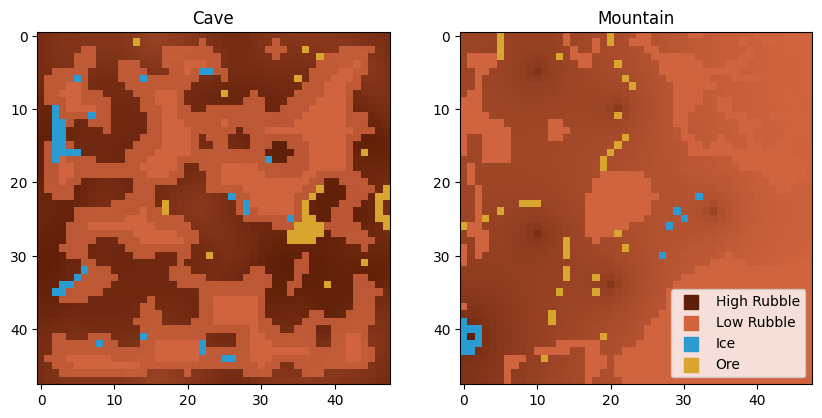
\includegraphics[width=1\linewidth]{images/intro_luxenv/map/resources.png}
    \captionsetup{justification=justified, singlelinecheck=false, width=1\linewidth, labelfont=bf}    
    \caption{Visual Representation of Lux 2D map types which exhibit unique layouts, each generated based on specific seeds \protect\footnotemark. In cave maps, resources are situated inside ravines, while mountain maps, presenting a more challenging terrain, hide resources beneath extensive rubble.}
    \label{fig:lux-map}
\end{figure}

\footnotetext{The maps were generated using seeds $560$ and $788$.}

\subsection{Early Game}
\label{subsec:early-game}

\noindent Each player will start the game by bidding on factory placement order, then alternating placing several factories and specifying their starting resources. Factory placement policies play a crucial role in speeding up the learning process within the game environment. By strategically situating units closer to resources, these policies establish a less cluttered and more conducive proximity environment, thereby promoting faster resource collection. Additionally, the introduction of bidding mechanisms enhances the competitive aspect of the game, compelling players to outbid one another for optimal factory spawn locations. Players are given starting resources for the bidding process. \textcolor{deepblue}{\autoref{fig:lux-map2}} shows map states after concluding the \textbdd{factory placement} and \textbdd{bidding tasks}.

\begin{figure}[htbp]
    \centering
    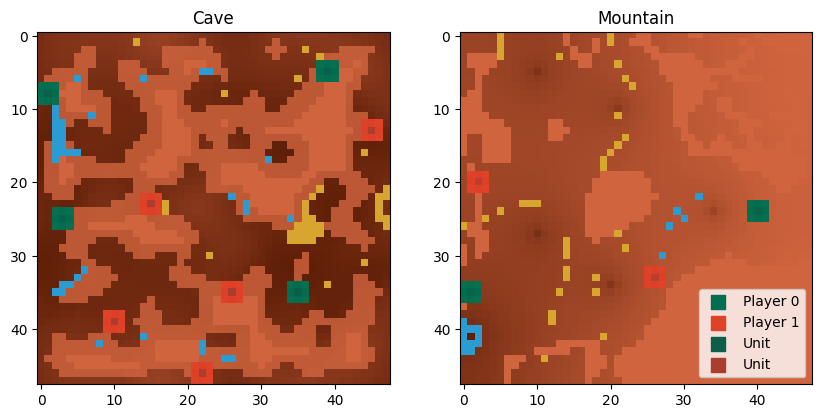
\includegraphics[width=1\linewidth]{images/intro_luxenv/map/factories_units.png}
    \captionsetup{justification=justified, singlelinecheck=false, width=1\linewidth, labelfont=bf}    
    \caption{Visual representation of a random factory placement policy on the two generated maps presented on \textcolor{deepblue}{\autoref{fig:lux-map}}. For further restrictions on factory placement and bidding, please refer to the more in-depth documentation \protect\footnotemark.}
    \label{fig:lux-map2}
\end{figure}

\footnotetext{Advanced specifications available on \href{https://github.com/Lux-AI-Challenge/Lux-Design-S2/blob/main/docs/advanced_specs.md}{GitHub.}}

\subsection{Resources}

\noindent The two kinds of raw resources shown in \textcolor{deepblue}{\autoref{fig:lux-map}}, Ice and Ore, can be refined by a factory into Water or Metal respectively. The raw resources are collected by Light or Heavy units and then dropped off once a unit transfers them to a friendly factory, which then automatically converts them into refined resources at a constant rate. Refined resources are used for growing Lichen, powering factories as well as building more units. For detailed conversion rates and restrictions on transferring resources, please refer to the documentation (\textcolor{deepblue}{\cite{lux-ai-season-2}}).

\subsection{Actions}
\label{subsec:lux-action}

\noindent Units and factories can perform actions at each turn, given certain conditions and enough power to do so. In general, all actions are simultaneously applied and are validated against the state of the game at the start of each turn (\cite{chen2023emergent}). Every turn, players can give an action to each factory and a queue of actions to each unit. Units always execute actions from an action queue, which is limited to a size of 20, while factories directly execute actions. Players can choose to repeat actions for $n$ times, which further complicates the action queue. Submitting a new action queue for a robot requires the robot to use additional power to replace it's current action queue. It costs an additional $1$ power, for light units and an additional $10$ power, for heavy units. For further information regarding action queue updates and repeat handling, please, refer to the documentation (\textcolor{deepblue}{\cite{lux-ai-season-2}}). There are six possible action types that are simplified for easier understanding on \textcolor{deepblue}{\autoref{fig:lux-actions}}.

\bigskip

\begin{figure}[htbp]
    \centering
    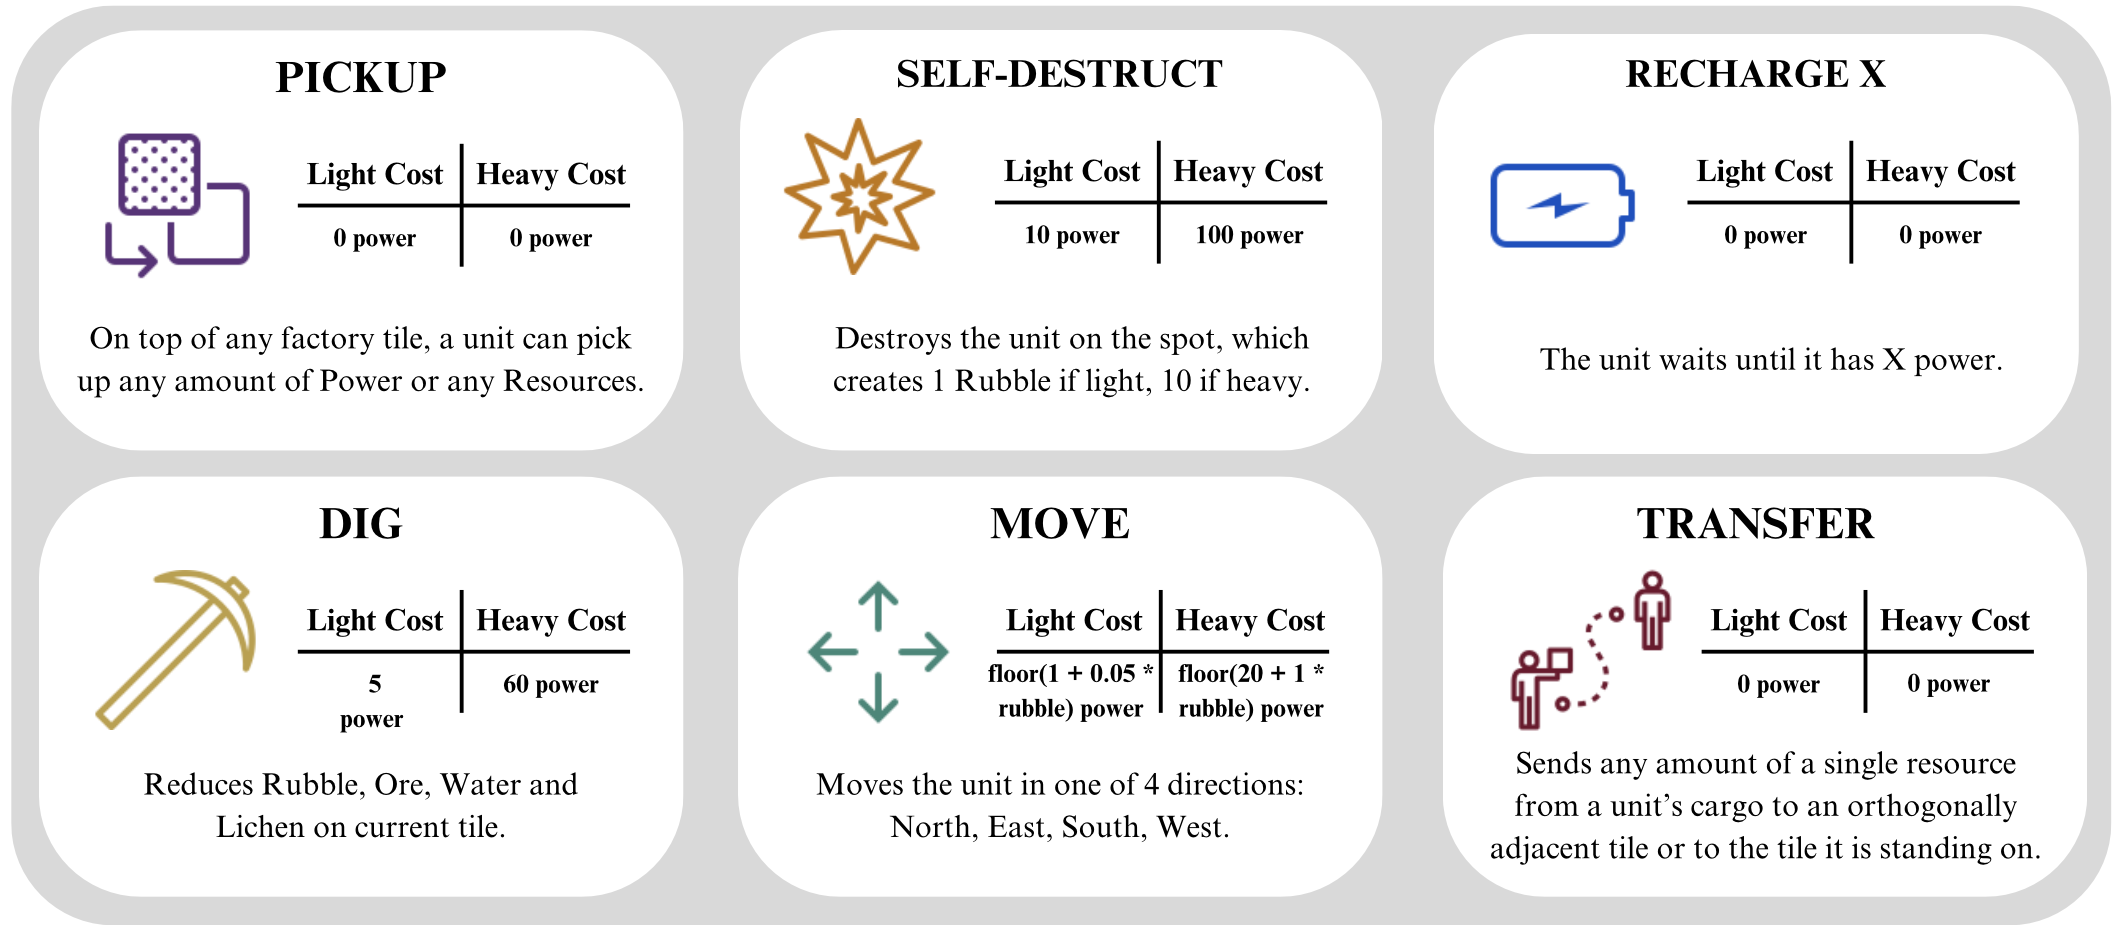
\includegraphics[width=1\linewidth]{images/intro_luxenv/action/action_space.png}
    \captionsetup{justification=justified, singlelinecheck=false, width=1\linewidth, labelfont=bf} 
    \caption{Simplified representation of all possible actions available in the Lux environment. Additional limits and restrictions are applied in the implementation of the engine (\textcolor{deepblue}{\cite{lux-ai-season-2}}).}
    \label{fig:lux-actions}
\end{figure}

\noindent A factory is a building that takes up $3\times3$ tiles of space. Units created from the factory will appear at the center of the factory. Factories can assume passive roles with fixed heuristic action generation, alongside active roles where actions are learned. The action vectors for both factories and units are 1D vectors. Given $n$ units and $m$ factories, predicting action vectors yields matrices of $n\times6$ and $m\times1$, respectively. The response template to the \textbdd{Lux engine} conforms to the format illustrated in \textcolor{deepblue}{\autoref{fig:lux-actions_ex}}.

\begin{figure}[htbp]
    \centering
    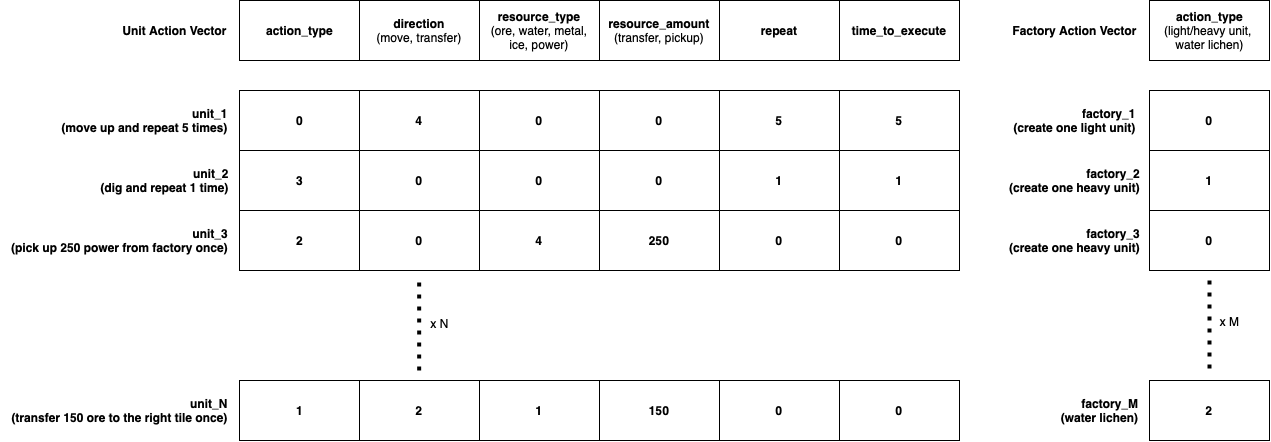
\includegraphics[width=1\linewidth]{images/intro_luxenv/action/action_example.png}
    \captionsetup{justification=justified, singlelinecheck=false, width=1\linewidth, labelfont=bf}
    \caption{Visual example of possible action vectors for both units and factories.}
    \label{fig:lux-actions_ex}
\end{figure}

\subsection{Rubble Dynamics}

\noindent Each square on the map has a rubble value, which affects how difficult that square is to move onto. Rubble value is an integer ranging from 0 to 100. Rubble can be removed from a square by a light or heavy unit by executing the dig action while occupying the square. This environment also has unit collisions. Units which move onto the same square on the same turn can be destroyed and add rubble to the square according to a list of extensive rules in the documentation (\textcolor{deepblue}{\cite{lux-ai-season-2}}).

\subsection{Night Cycles}

\noindent Night cycles are introduced as a complexity measure in the Lux Environment to enhance dynamism and continual change. The environment alternates between \textbdd{day cycles}, which last 30 steps, and \textbdd{night cycles}, which are 20 steps long. This alternation continues until the episode concludes at 1000 steps. During night cycles, the recharging capability of units is stopped, although factories continue to produce power without change (\textcolor{deepblue}{\cite{lux-ai-season-2}; \cite{chen2023emergent}}).

\subsection{Win Condition}
\label{sec:wincondition}

\noindent A game can be resolved in four possible ways:

\begin{itemize}[itemsep=1pt, parsep=0pt]
\item 
In the event that all factories belonging to a player explode, the opposing player is declared the winner.
\item 
If both players lose their last factories in the same step, the game ends in a draw.
\item If each player maintains at least one operational factory, victory in the Lux AI environment is determined by the quantity of Lichen tiles under their control. Lichen watering serves a dual purpose: establishing victory conditions and generating additional power for factories. Due to the intricate nature of power calculations and lichen watering dynamics, we advise consulting the detailed documentation for further understanding (\textcolor{deepblue}{\cite{lux-ai-season-2}}).
\item If the quantity of owned Lichen tiles match, the game concludes in a draw.
\end{itemize}
\noindent






